\documentclass{sigchi}
%% \documentclass{sig-alternate-05-2015}

% Use this command to override the default ACM copyright statement
% (e.g. for preprints).  Consult the conference website for the
% camera-ready copyright statement.

%% EXAMPLE BEGIN -- HOW TO OVERRIDE THE DEFAULT COPYRIGHT STRIP -- (July 22, 2013 - Paul Baumann)
% \toappear{Permission to make digital or hard copies of all or part of this work for personal or classroom use is      granted without fee provided that copies are not made or distributed for profit or commercial advantage and that copies bear this notice and the full citation on the first page. Copyrights for components of this work owned by others than ACM must be honored. Abstracting with credit is permitted. To copy otherwise, or republish, to post on servers or to redistribute to lists, requires prior specific permission and/or a fee. Request permissions from permissions@acm.org. \\
% {\emph{CHI'14}}, April 26--May 1, 2014, Toronto, Canada. \\
% Copyright \copyright~2014 ACM ISBN/14/04...\$15.00. \\
% DOI string from ACM form confirmation}
%% EXAMPLE END -- HOW TO OVERRIDE THE DEFAULT COPYRIGHT STRIP -- (July 22, 2013 - Paul Baumann)

% Arabic page numbers for submission.  Remove this line to eliminate
% page numbers for the camera ready copy
% \pagenumbering{arabic}

% Load basic packages
\usepackage{balance}  % to better equalize the last page
\usepackage{graphics} % for EPS, load graphicx instead 
\usepackage[T1]{fontenc}
\usepackage{txfonts}
\usepackage{mathptmx}
\usepackage[pdftex]{hyperref}
\usepackage{color}
\usepackage{booktabs}
\usepackage{textcomp}
% Some optional stuff you might like/need.
\usepackage{microtype} % Improved Tracking and Kerning
% \usepackage[all]{hypcap}  % Fixes bug in hyperref caption linking
\usepackage{ccicons}  % Cite your images correctly!
% \usepackage[utf8]{inputenc} % for a UTF8 editor only

% If you want to use todo notes, marginpars etc. during creation of your draft document, you
% have to enable the "chi_draft" option for the document class. To do this, change the very first
% line to: "\documentclass[chi_draft]{sigchi}". You can then place todo notes by using the "\todo{...}"
% command. Make sure to disable the draft option again before submitting your final document.
\usepackage{todonotes}

% Paper metadata (use plain text, for PDF inclusion and later
% re-using, if desired).  Use \emtpyauthor when submitting for review
% so you remain anonymous.
\def\plaintitle{Hierarchical modeling in education performance prediction}
\def\plainauthor{First Author, Second Author, Third Author,
  Fourth Author, Fifth Author, Sixth Author}
\def\emptyauthor{}
\def\plainkeywords{Authors' choice; of terms; separated; by
  semicolons; include commas, within terms only; required.}
\def\plaingeneralterms{Documentation, Standardization}

% llt: Define a global style for URLs, rather that the default one
\makeatletter
\def\url@leostyle{%
  \@ifundefined{selectfont}{
    \def\UrlFont{\sf}
  }{
    \def\UrlFont{\small\bf\ttfamily}
  }}
\makeatother
\urlstyle{leo}

% To make various LaTeX processors do the right thing with page size.
\def\pprw{8.5in}
\def\pprh{11in}
\special{papersize=\pprw,\pprh}
\setlength{\paperwidth}{\pprw}
\setlength{\paperheight}{\pprh}
\setlength{\pdfpagewidth}{\pprw}
\setlength{\pdfpageheight}{\pprh}

% Make sure hyperref comes last of your loaded packages, to give it a
% fighting chance of not being over-written, since its job is to
% redefine many LaTeX commands.
\definecolor{linkColor}{RGB}{6,125,233}
\hypersetup{%
  pdftitle={\plaintitle},
% Use \plainauthor for final version.
%  pdfauthor={\plainauthor},
  pdfauthor={\emptyauthor},
  pdfkeywords={\plainkeywords},
  bookmarksnumbered,
  pdfstartview={FitH},
  colorlinks,
  citecolor=black,
  filecolor=black,
  linkcolor=black,
  urlcolor=linkColor,
  breaklinks=true,
}

% create a shortcut to typeset table headings
% \newcommand\tabhead[1]{\small\textbf{#1}}

% End of preamble. Here it comes the document.
\begin{document}

\title{\plaintitle}

\numberofauthors{1}
\author{%
  \alignauthor{James Nguyen\\
    \affaddr{Georgia Tech}\\
    \affaddr{Atlanta, GA, USA}\\
    \email{cuong.nguyen@gatech.edu}}\\
}


\maketitle

\begin{abstract}
  Recent advances in Machine Learning and Data Mining enable new
  branches of educational research to thrive, particularly e-learning and data
  capturing through e-learning systems. \cite{romero2010educational}
  Academic performance research benefits strongly from this trend
  through better data and models. In this paper,
  I investigate \textbf{hierarchical models} - a flexible family of advanced
  parametric models - that could achieve not only high \textbf{out-of-sample prediction
  power} but also \textbf{meaningful confidence intervals} for \textbf{statistical
  inference}. Reviews and empirical comparisons versus traditional machine
  learning methods on an educational dataset are also provided in details.
  
\end{abstract}

\category{H.5.m.}{Information Interfaces and Presentation
  (e.g. HCI)}{Miscellaneous} \category{J.4.m.}{Computer Applications}
{SOCIAL AND BEHAVIORAL SCIENCES} \category{G.3.m.}{Mathematics of computing}{Probability and
  Statistics - Multivariate statistics} \category{I.5.1.m.}{Computing methodologies}{Pattern Recognition - Models}

\keywords{Parametric Models; Education Research; E-learning; Student Performance; Predictive
  Modeling; Statistical Inference; Bayesian computation; STAN; Hierarchical
  Models; MCMC; Confidence
  Interval; Prediction Interval}

\section{Historical review of Education research}
The paper reviews the evolution of quantitative predictive methods in
education research to motivate interest in advanced parametric methods.

\subsection{Parametric Statistical Models}
Traditionally, research in education and educational
policies have applied similar quantitative methods to those used in the social sciences
\cite{gelman2009quantitative}, because the main goal of these
educational inquiries is to \textbf{establish causal effects}. \textbf{Parametric}, sparse models which allow ease of \textbf{hypothesis testing}
therefore are both prevalent and important, while black-box,
flexible predictive models are not popular. \cite{teo2014handbook}

Some parametric models offer \textbf{prediction capability} with 
\textbf{confidence intervals (CIs)}. However, unlike causality testing, prediction only take secondary roles in traditional education research,
so these models are not built to optimize for out-of-sample accuracy. \cite{romero2010educational}.

\subsection{Recent Machine learning methods}
Advances in EdTech enable new
branches of educational research to thrive, particularly \textbf{intelligent learning systems}. \cite{romero2010educational}
New ways of generating data and richer features through e-learning systems enable researchers to build better predictive models. People apply more modern methods on these datasets;
\textbf{ensembles, neural nets} and \textbf{SVMs} are the most common methods
when optimizing for \textbf{out-of-sample accuracy}. \cite{shahiri2015review}, \cite{amrieh2016mining} 

The body of work that apply predictive ML methods
on educational data tends to \textit{weight practicality more than interpretability}, and
they do not focus on answering traditional inference questions. \cite{romero2010educational, meier2016predicting}

\section{Research goal and methodology}
Could we build flexible predictive models
that offer \textit{not only high out-of-sample prediction
  power but also meaningful confidence intervals for statistical
  inference.}? A family of advanced parametric models that could satisfy this
demand is \textbf{hierarchical models} - we will investigate their construction
process and predictive power in this paper.

\subsection{Hierarchical modeling in education research}
Hierarchical models offer a balance between 
predictive accuracy and interpretability. \textit{\textbf{Hierarchical models are particularly suitable for
educational research, because education data are generally collected
from a hierarchy.}} \cite{
skrondal2009prediction, kaplan2016causal} 

For example, you can have performance
scores for students in a
state, at different districts, different schools within the same district, different
class levels within the same school etc. Of course, if the data are generated in
a true controlled fashion with balanced groups representation across all
covariates, then we can do a pooled t-test, but these are survey or
longitudinal data with known \textbf{biases} and \textbf{imbalances}. \cite{konig2017bayesian}

There are few studies focusing on \textit{hierarchical models in academic performance}
\cite{tsai2015hierarchical, subedi2015measuring}, and there is no current study that focuses
on building a highly predictive hierarchical model first before interpreting
statistical significance.

\subsection{Bayesian Techniques in Hierarchical modeling}
Fitting hierarchical model is one of the
major usage of \textbf{Bayesian techniques}. Previously, due to
computational complexity of the sampling algorithms in these Bayesian techniques, building hierarchical models are hard.
However, recent advances in hardware and software have opened up these techniques to a wider range of social science problems. \cite{carpenter2017stan}

\section{Data overview}
In coming sections, this research builds hierarchical models on a student
performance dataset
and compares those hierarchical models' predictive power against
state-of-the-art tree-based models built on the same data.


The reference educational dataset in \cite{amrieh2016mining} is collected from a learning management system (LMS) using an activity tracker. This learning system monitors learning progress like reading an article or watching a training video. 

The data consist of \textbf{480 student records} and \textbf{17 features}, with final performance as the desired predictive outcome - \ref{fig:gender_outcome}. 

\subsection{Features}
The features are classified into three major categories:

\begin{itemize}
	\item Demographic: gender and nationality etc. - Fig. \ref{fig:gender_outcome}, \ref{fig:nationality_fig}
	\item Academic: topic, grade level and section etc. - Fig. \ref{fig:topic_bar}
	\item Behavioral: raised hand on class, visited resources, answering survey by parents, and school satisfaction - Fig \ref{fig:vresources_outcome}
\end{itemize}


\begin{figure}
	\centering
		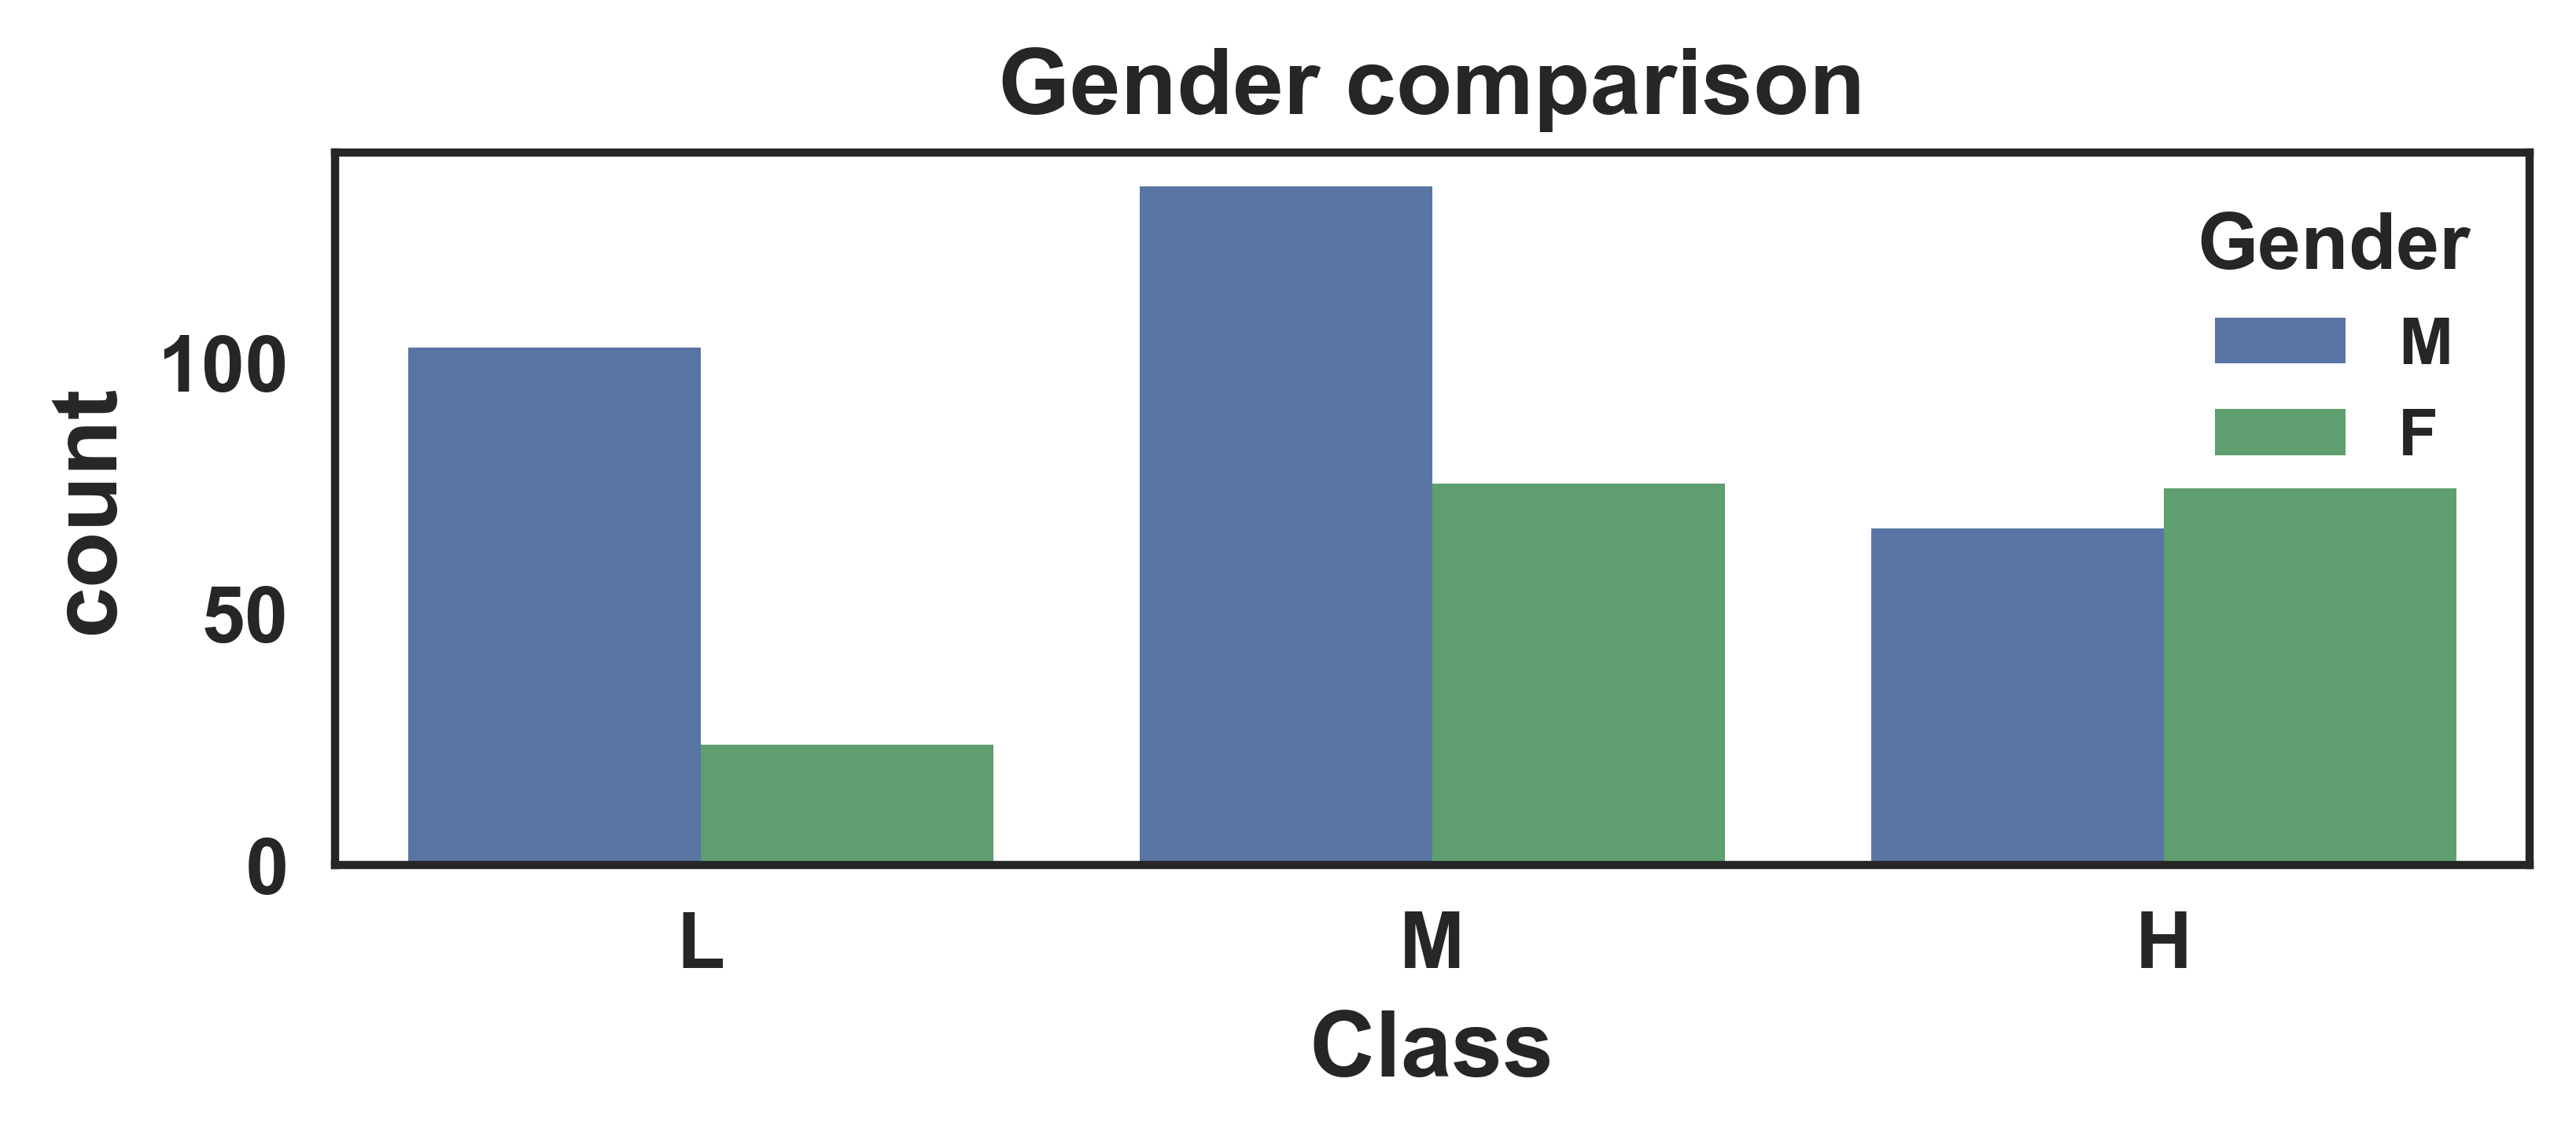
\includegraphics[width=0.95\columnwidth]{figures/gender_outcome.png}
		\caption{
			Women tend to perform better than men on average.
		}~\label{fig:gender_outcome}	
	
	\centering
	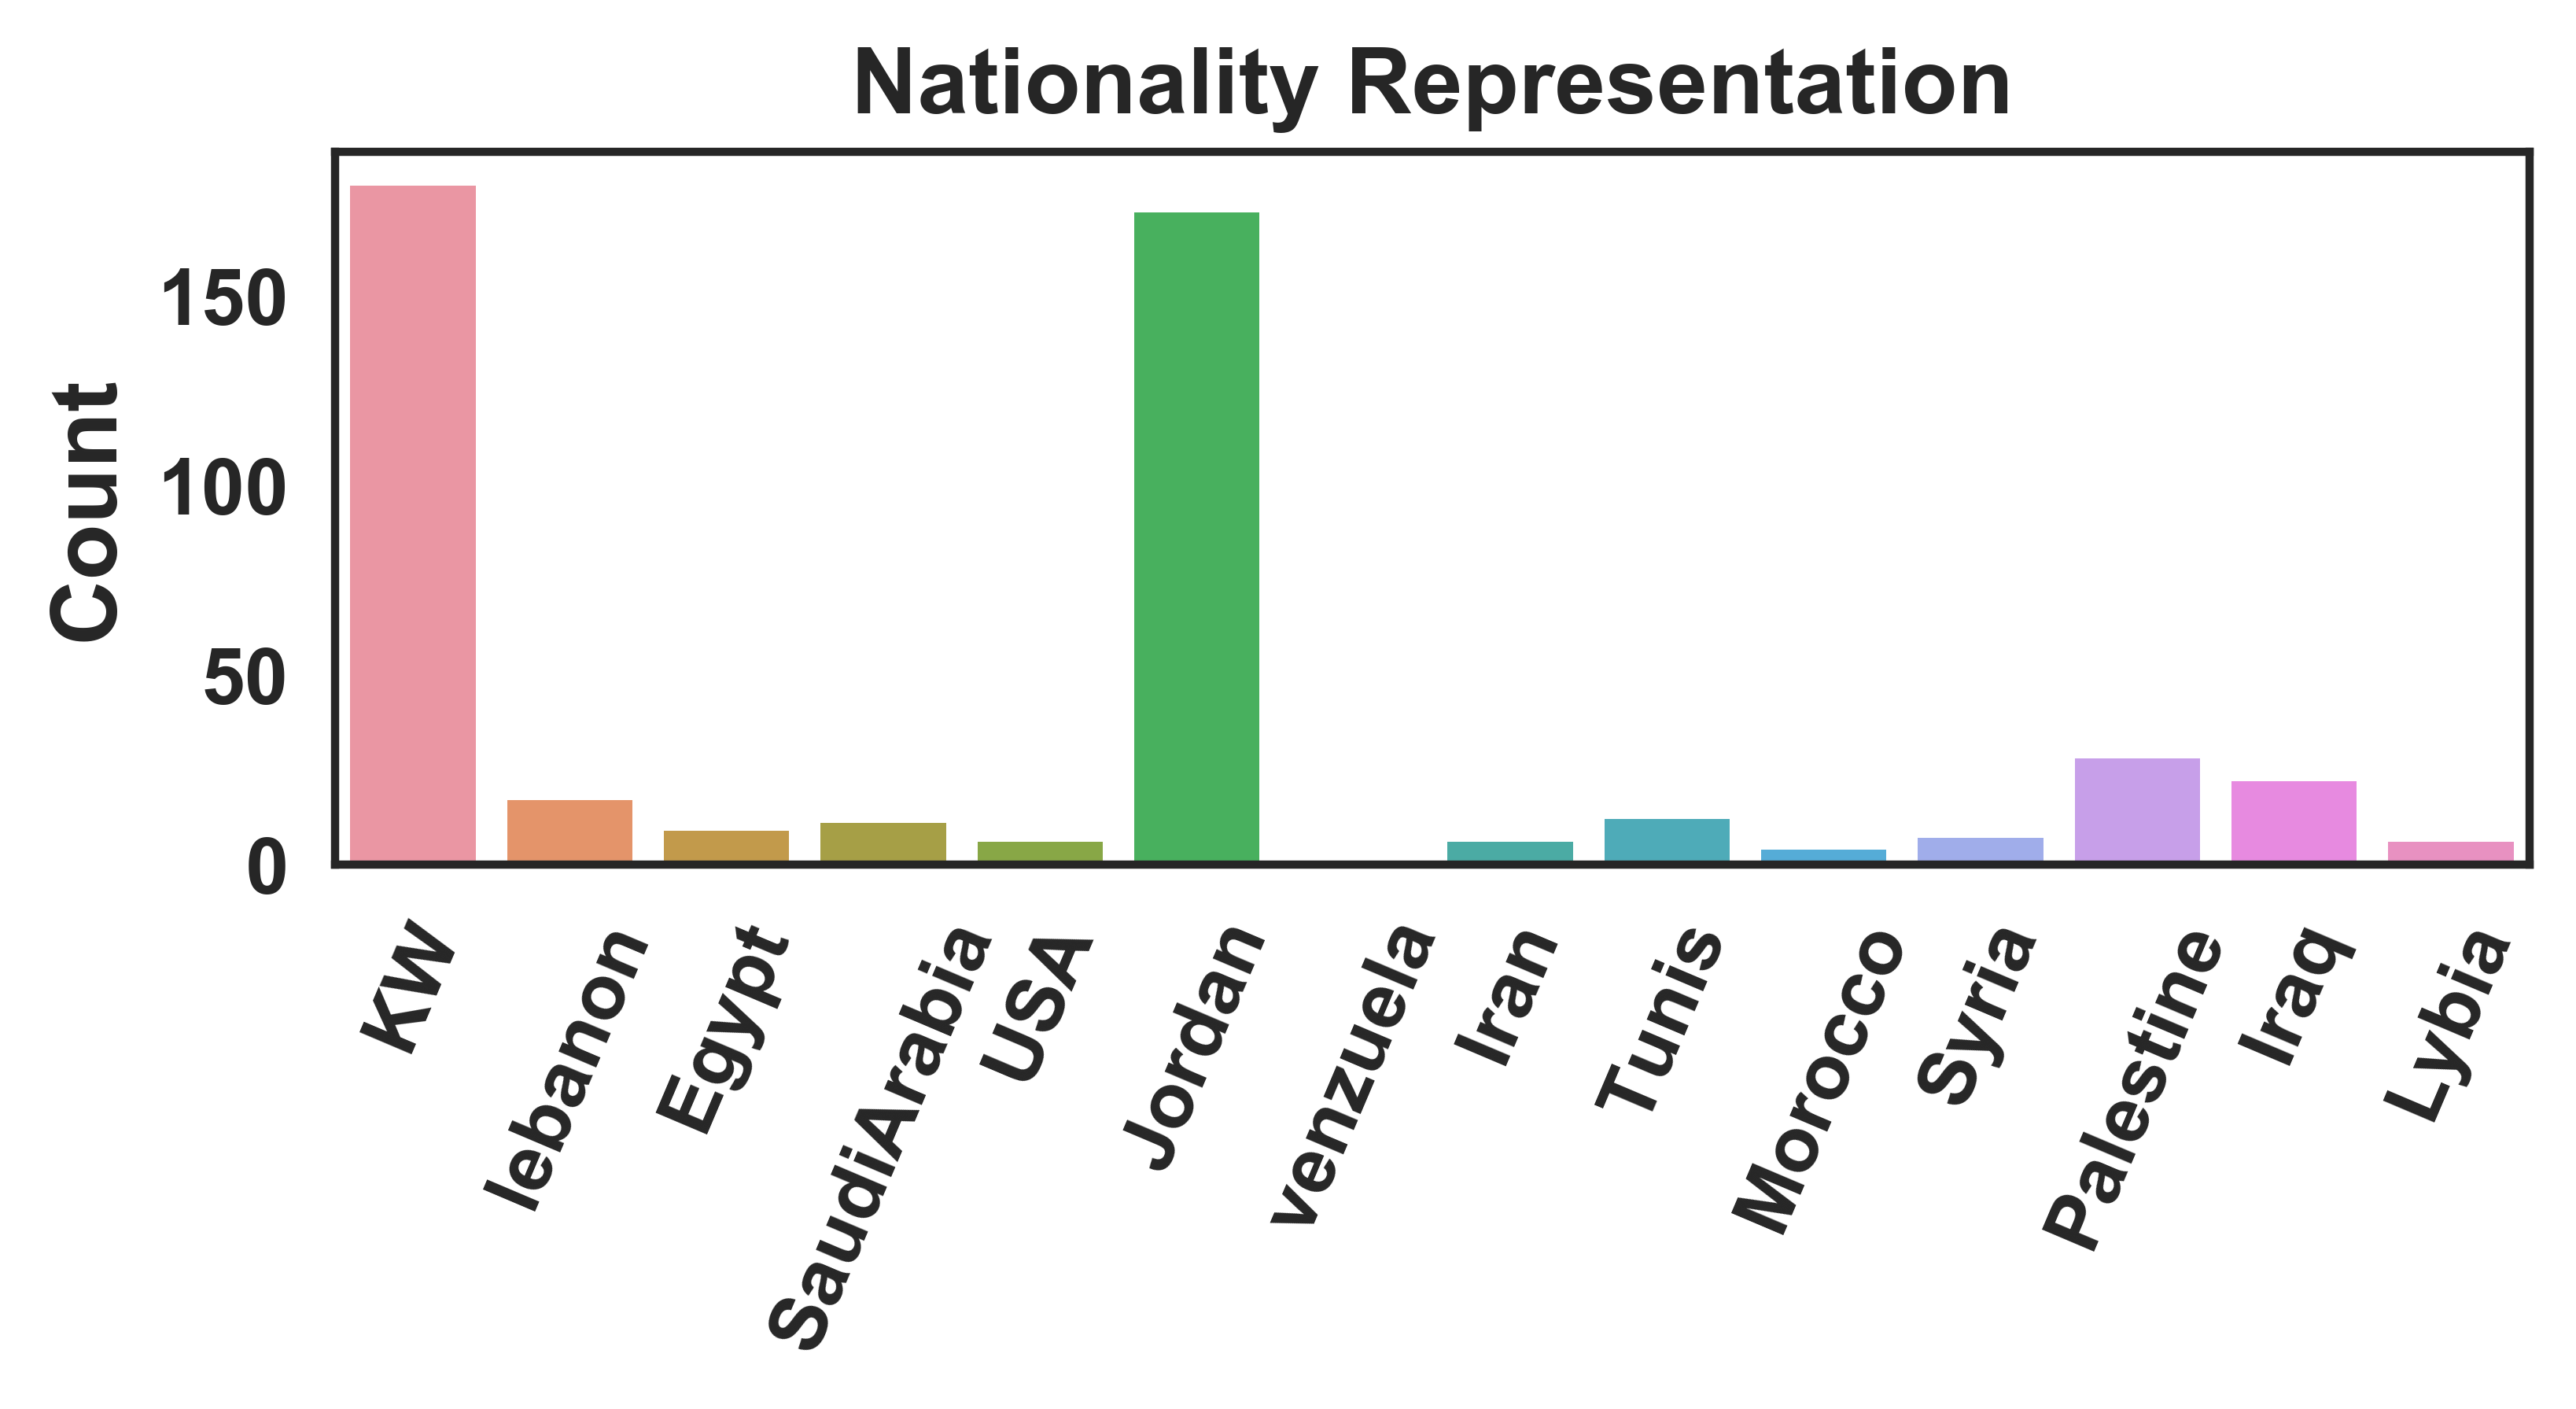
\includegraphics[width=0.95\columnwidth]{figures/nationality_bar.png}
	\caption{
		The students come from different origins: 179 are from Kuwait, 172 are from Jordan, and smaller groups < 30 from Palestine, Iraq, Lebanon, Tunis, Saudi Arabia, Egypt, Syria etc.
}~\label{fig:nationality_fig}


	\centering
	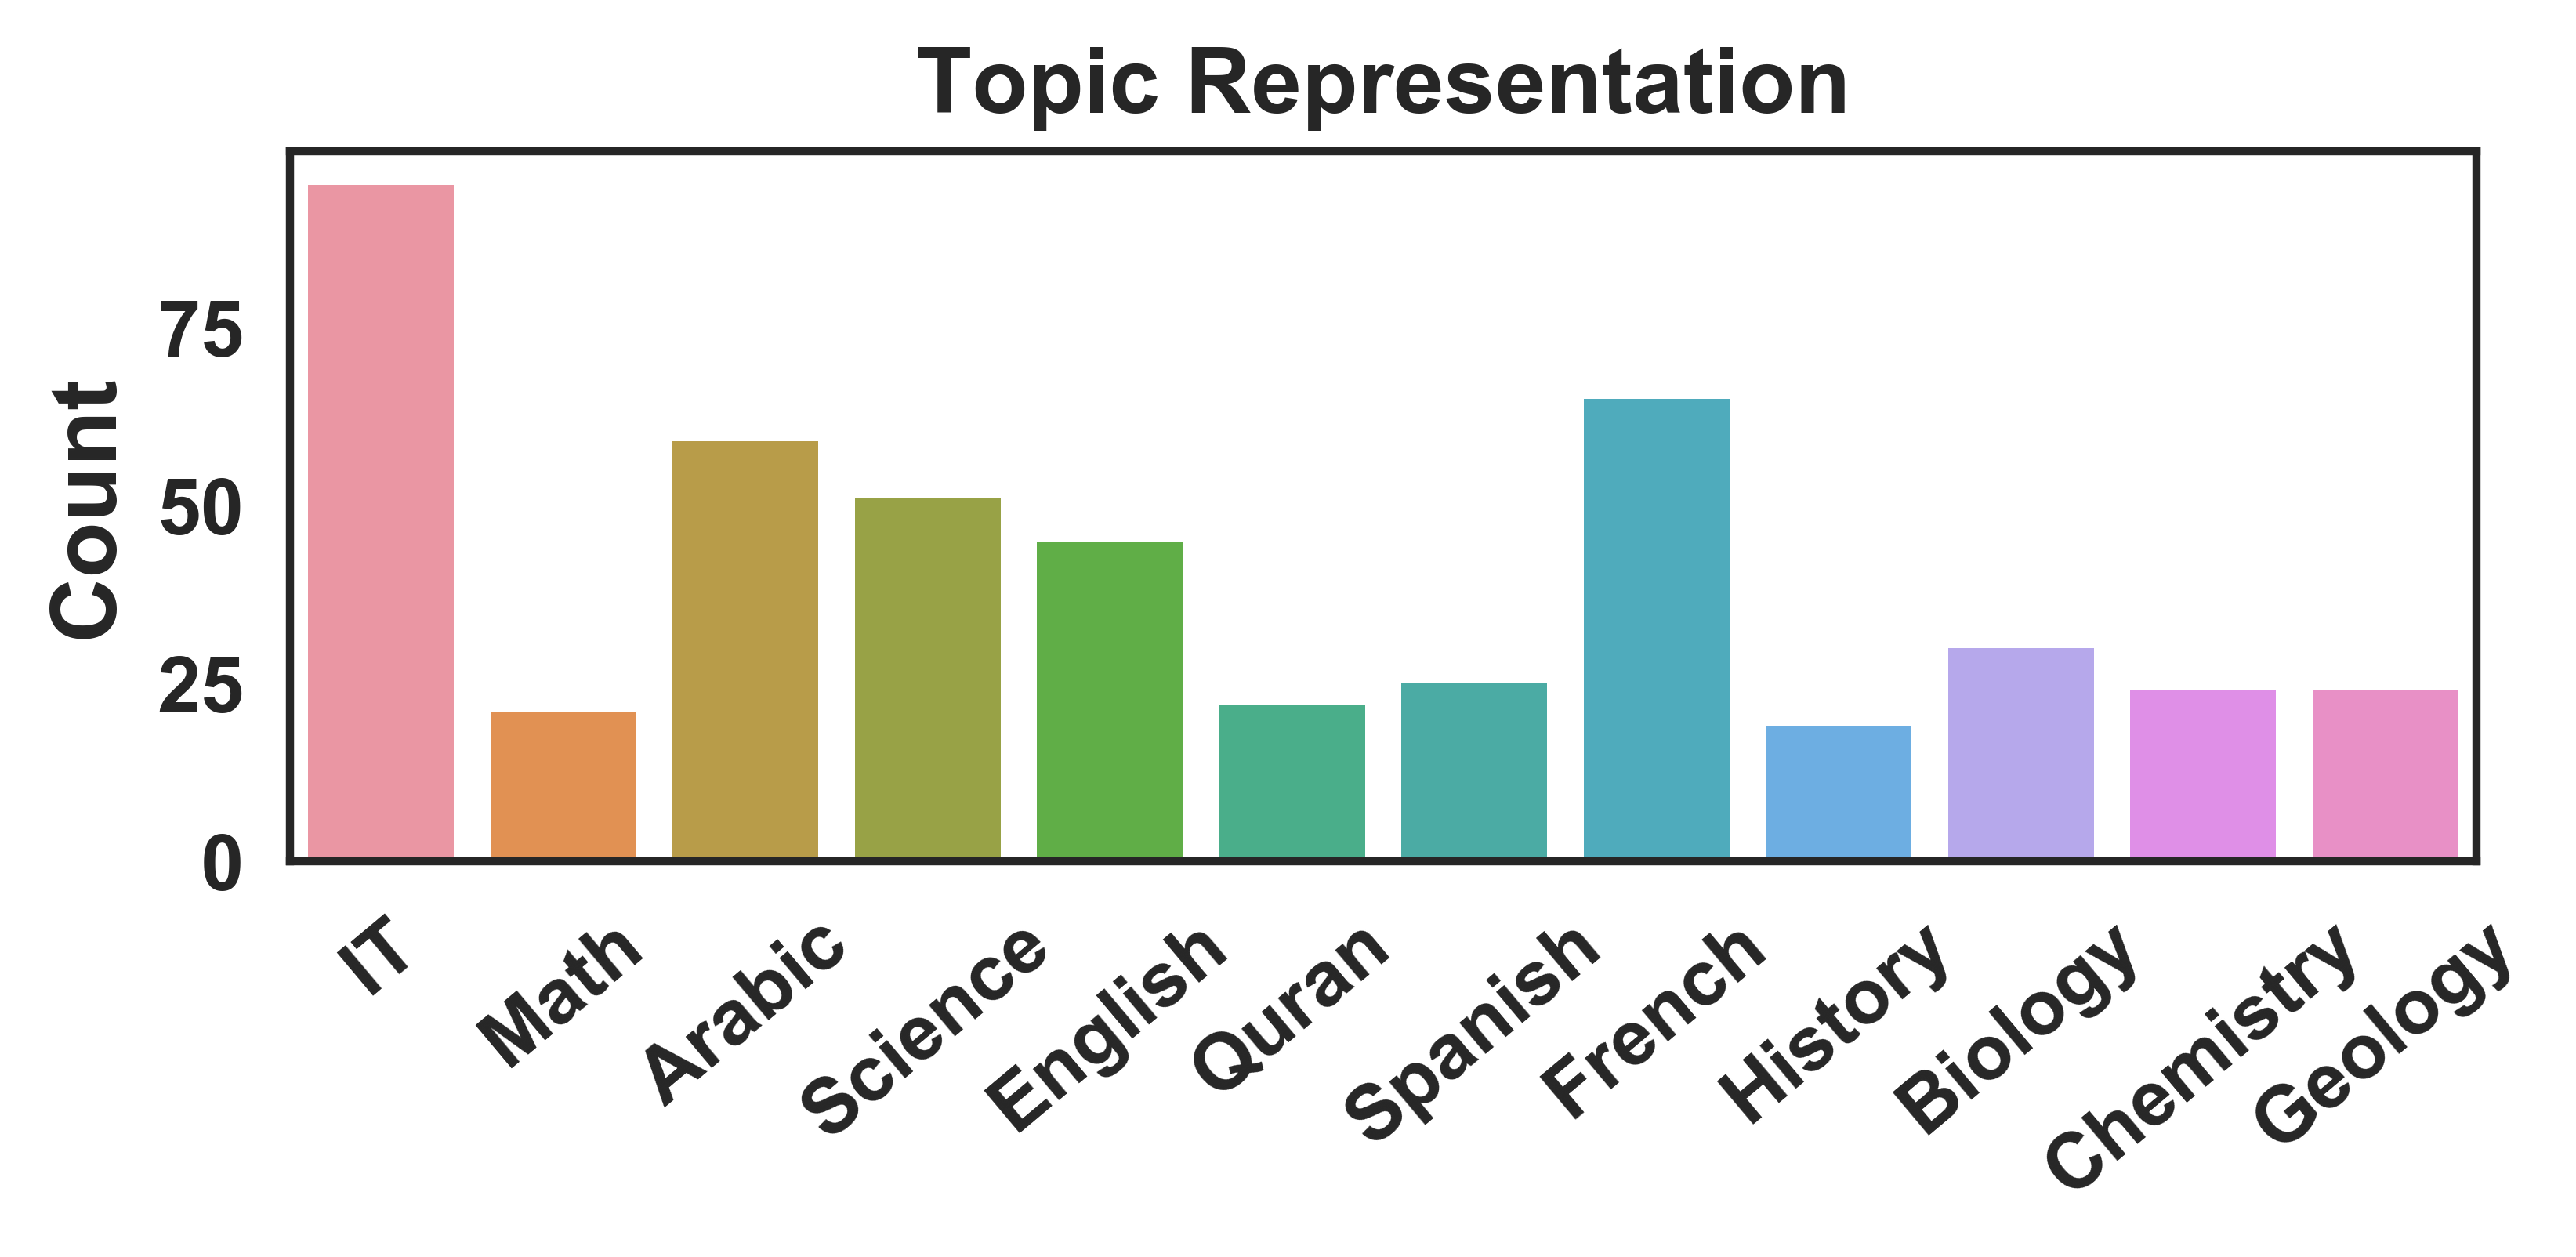
\includegraphics[width=0.95\columnwidth]{figures/topic_bar.png}
	\caption{
		Multiple topics included - this feature is also unbalanced.
	}~\label{fig:topic_bar}

	\centering
	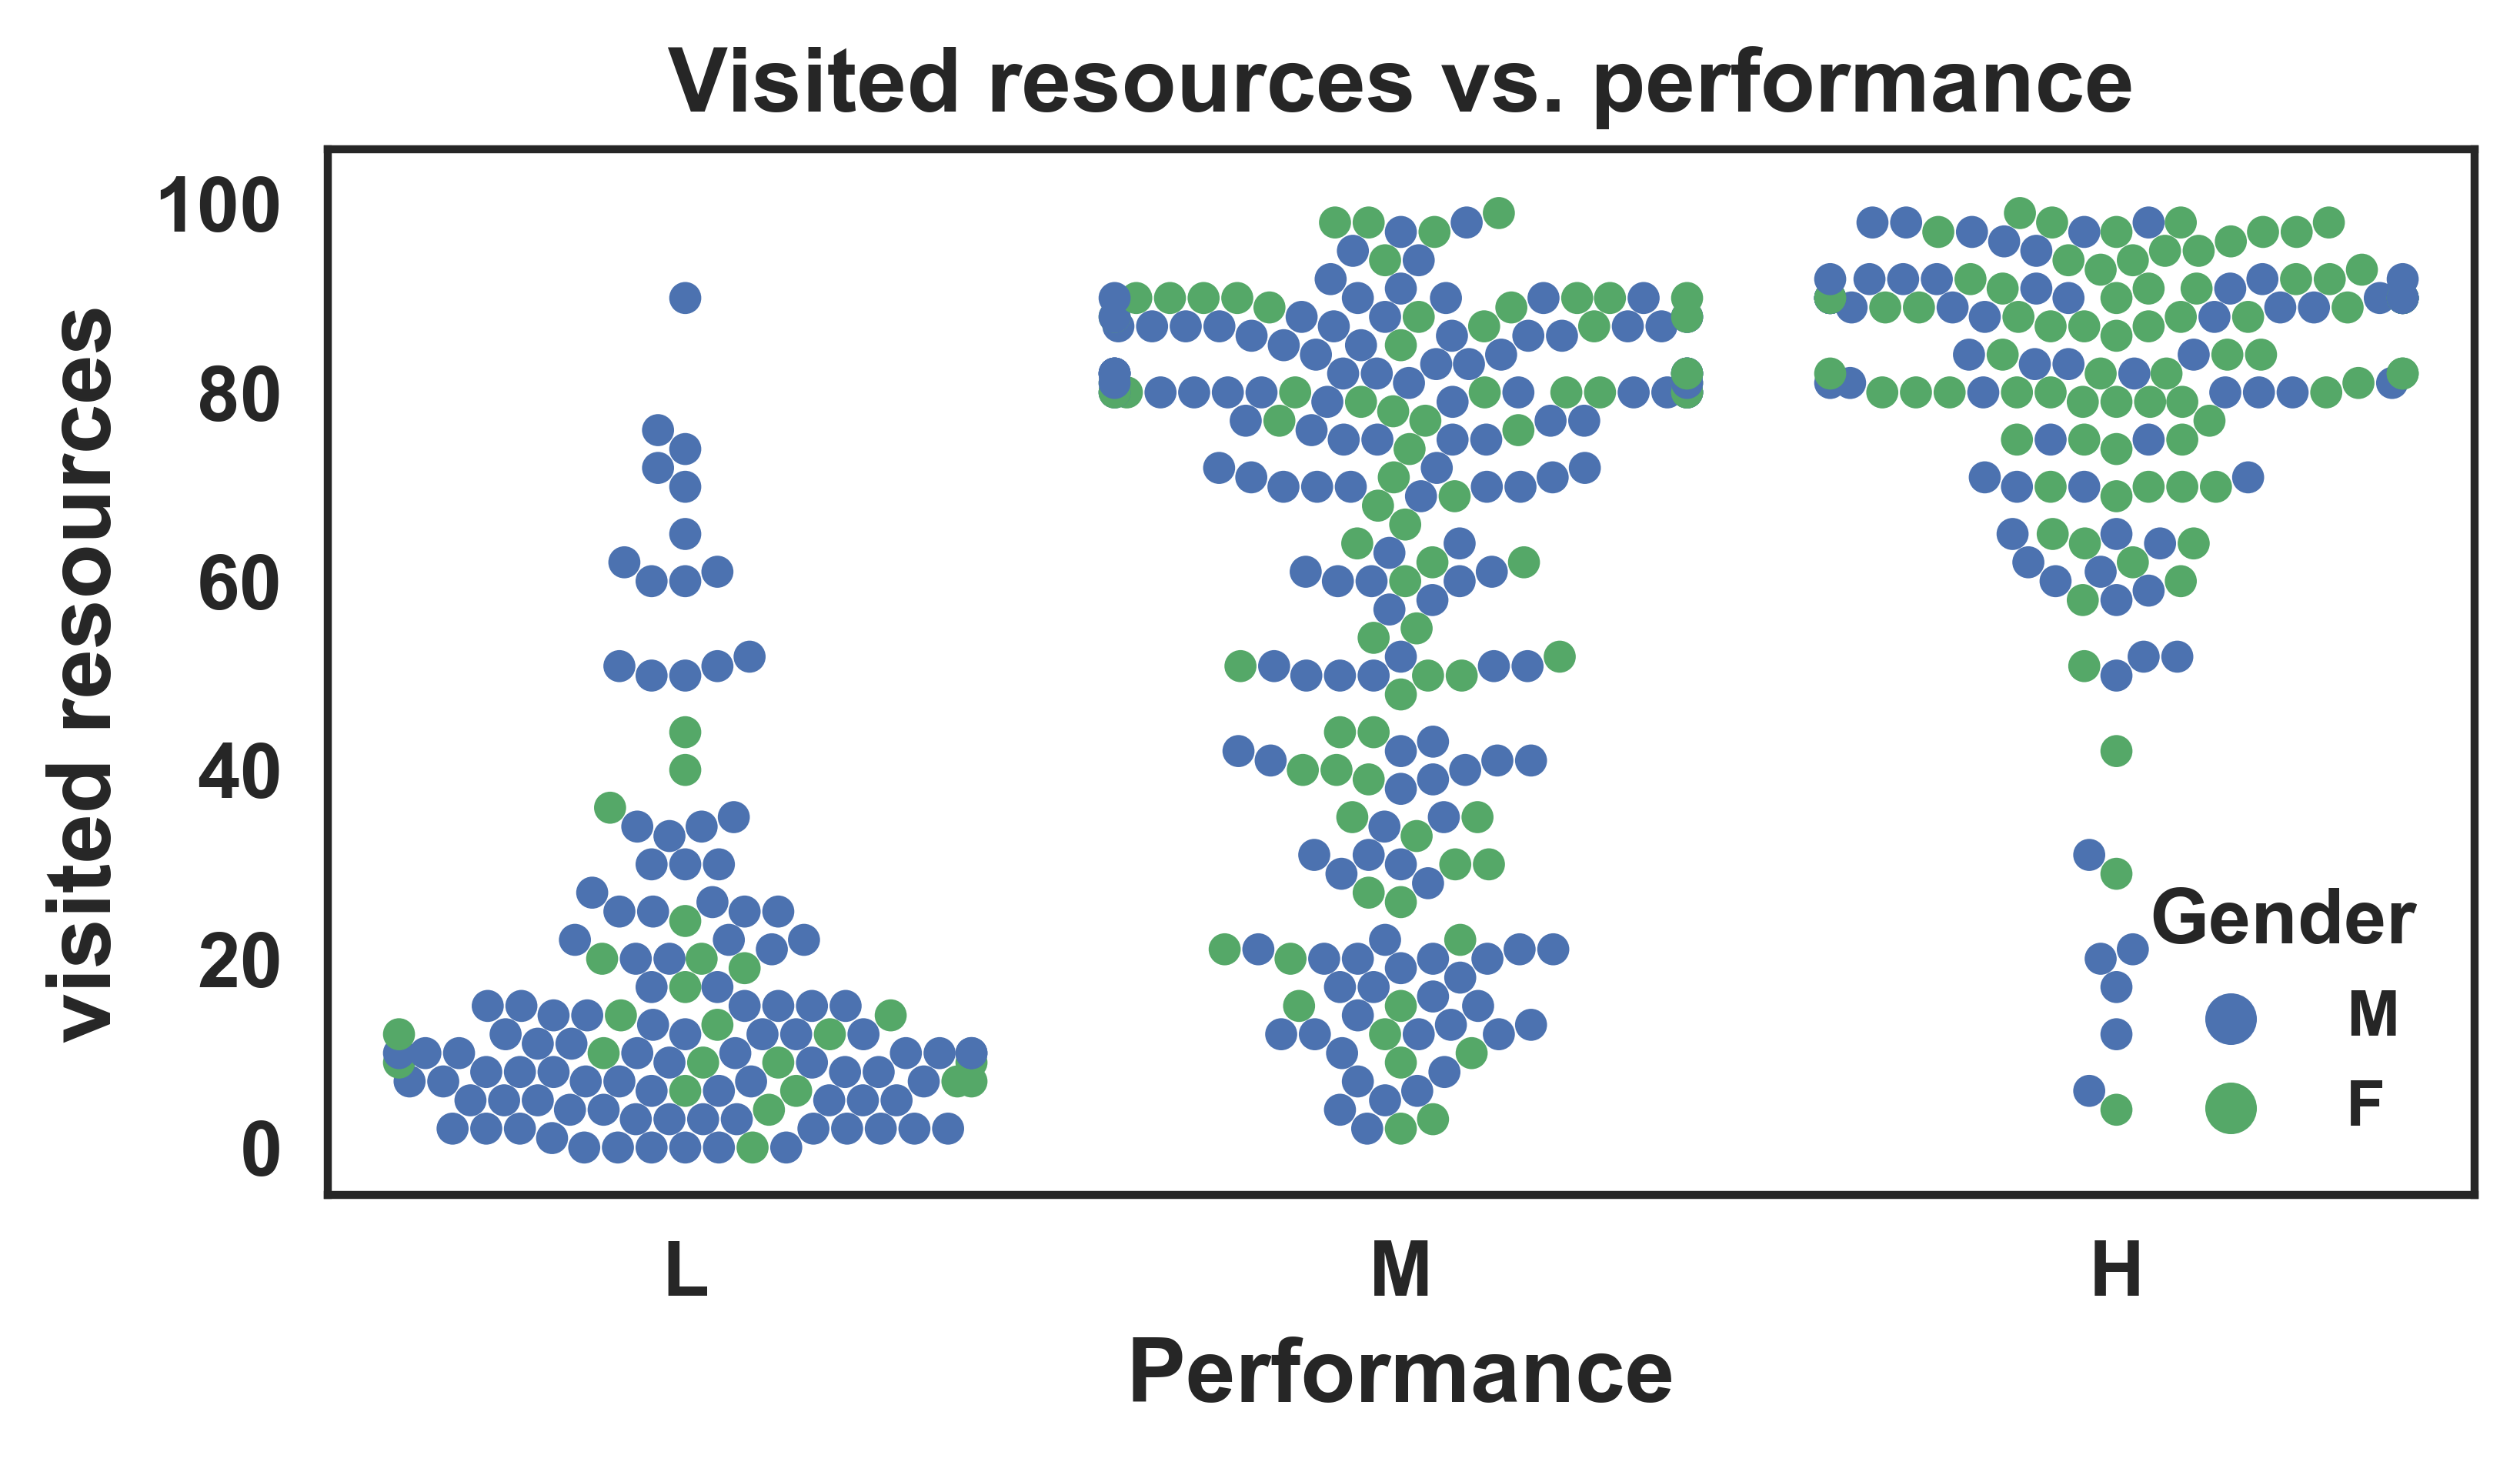
\includegraphics[width=0.95\columnwidth]{figures/vresources_outcome.png}
	\caption{
		Tendency to visit resources is a \textit{behavioral feature} - only made available by E-learning systems. This plot shows that students who received a lower grade (L) visited fever resources than students that scored a M or H grade. Additionally, women who received a high mark (H) almost exclusively visited a lot of the on-line resources.
	}~\label{fig:vresources_outcome}	
\end{figure}


\subsection{Reference tree-based models}
Reference state-of-the-art tree-based models are taken from \textbf{Amrieh
et. al.} \cite{amrieh2016mining}, where the authors built learners on this data and show that ensemble
models achieve strong out-of-sample prediction. I reproduced their results using \textbf{25pct} of data as hold-out test set with accuracy listed in table \ref{tab:accuracy_results}.

\subsection{Shortcomings of tree-based/black-box methods}
For inference, the predicted values from tree-based/black-box models do not provide useful
information that aids decision making, e.g. confidence intervals and
significance of contributing factors. 
\cite{efron2016computer, meier2016predicting} E.g, by topic, the dataset in
\cite{amrieh2016mining} is unbalanced (\textbf{Fig. \ref{fig:topic_bar}}): \textbf{IT} has 95 students
vs. \textbf{Maths} has 21 students, so performance prediction for a new Maths
student should be a lot less certain than that of a new IT
student. Meanwhile, none of the blackbox models can reflect such confidence
adjustments based on their predictive values.

\pagebreak
\begin{table}
	\centering
	\begin{tabular}{l r}
		% \toprule
		
		{\small\textit{Model}} & {\small \textit{Accuracy}} \\
		\midrule
		Decision Tree                & 0.77    \\
		Random Forest                & 0.83    \\
		\textbf{Hierarchical Topic x Gender}  & \textbf{0.89}    \\
		Hierarchical Topic x Country & 0.89    \\
		&     \\
		% \bottomrule
	\end{tabular}
	\caption{
		Hierarchical models do better than both decision tree and random forest for out-of-sample prediction.
		The best hierarchical model (bold) accounts for groups interactions between Topics, Student Gender and 
		responsible Parent Gender.  	
	}~\label{tab:accuracy_results}
\end{table}


\section{Model building and assumptions}
This section walks through the parameterization of hierarchical models used, the model assumptions and their justifications. For a quick recap of hierarchical models and visualization, see Figure \ref{fig:hierarchy}; a more detailed treatment is available in \cite{gelmanbayesian}.

\begin{figure}
	\centering
	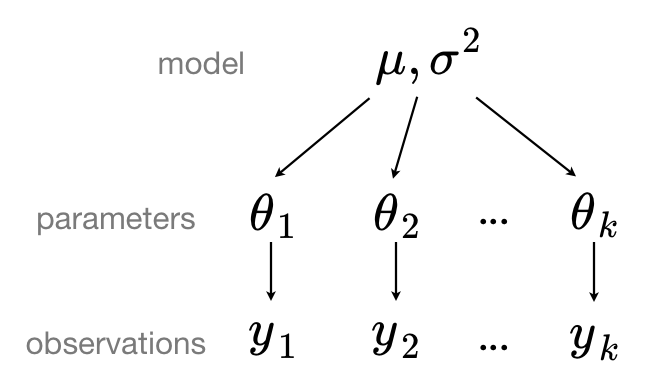
\includegraphics[width=0.95\columnwidth]{figures/hierarchy.png}
	\caption{
		In a hierarchical model, we see data at both individual-level ($\protect y_{t}$) and at group-level. Group-level parameters themselves ($\protect\theta_{i}$) are viewed as a sample from a distribution governed by hyper-parameters ($\protect\mu$ and $\protect\sigma$). 
		Thus, we view $\protect\theta_{i}$ as being neither entirely different or exactly the same - this is \textit{partial pooling}. 
	}~\label{fig:hierarchy}	
	
\end{figure}
 
\subsection{Hierarchy specifications} 
Figure \ref{fig:hierarchy} shows how we could view natural groups in the dataset such as Topics, Nationality or Gender as one level above the individual students. Each of these groups has its own average/parameter ($\theta_{i}$), but the groups' averages are related to each others - \textbf{partial pooling}. Partial pooling is very useful in dealing with unbalanced data, where some categories have only a few samples and we must borrow inference/prediction from other groups' parameters - e.g. Topics in Figure \ref{fig:topic_bar}.


\subsection{Model parameterization} 
At the data level, we have the logistic regression:
\[ Pr(y_{i} = 1 ) = logit^{-1}(X_{i}\theta_{j[i]}),  \; \text{for i=1,...,n  } \; \; (1) \] 

Where $\mathbf{X}$ is the matrix of individual-level features and $j[i]$ indexes the Topic/Gender groups that student $i$ belongs to. 


The group-level coefficients $\theta_{j}$ follows another distribution:

\[ \theta_{j} \; \mathbf{\texttildelow} \; Gaussian(\mu, \sigma^2_{\theta}),  \; \text{for j=1,..., 48  (48 groups)}  \; \; (2)\] 

Where $\mu$ is the vector of group-level average per features and $\sigma^2_\theta$ governs how much variability we expect in group-level coefficient $\theta_{j}$. The model for $\theta_{j}$ in (2) allows us to include all 48 groups in the full model without worrying about collinearity, and this two-level parameterization gives the model the name "hierarchical".

Several hierarchies types and depths are explored, but for this data, I found a simple 1-level hierarchy of \textbf{Topic x Student Gender x Parent Gender} interaction groups perform the best.



\subsection{Model performance}
One caveat for this dataset is that we actually need \textbf{2} logistic models specified by Equation \textbf{(1)} above, because we must classify \textbf{Low vs. Medium/High} and \textbf{High vs. Medium+Low} separately then combine the predictions for a 3-outcome target.

The out-of-sample accuracy of the hierarchical models outperform reference tree-based models in \cite{amrieh2016mining} - shown in Table \ref{tab:accuracy_results}. Not only that, this type of models can also make use of the \textbf{partial pooling} concept to predict outcomes for observations from a new group - by using the group average $\mu$ \cite{gelmanbayesian}.

\begin{figure}
	\centering
	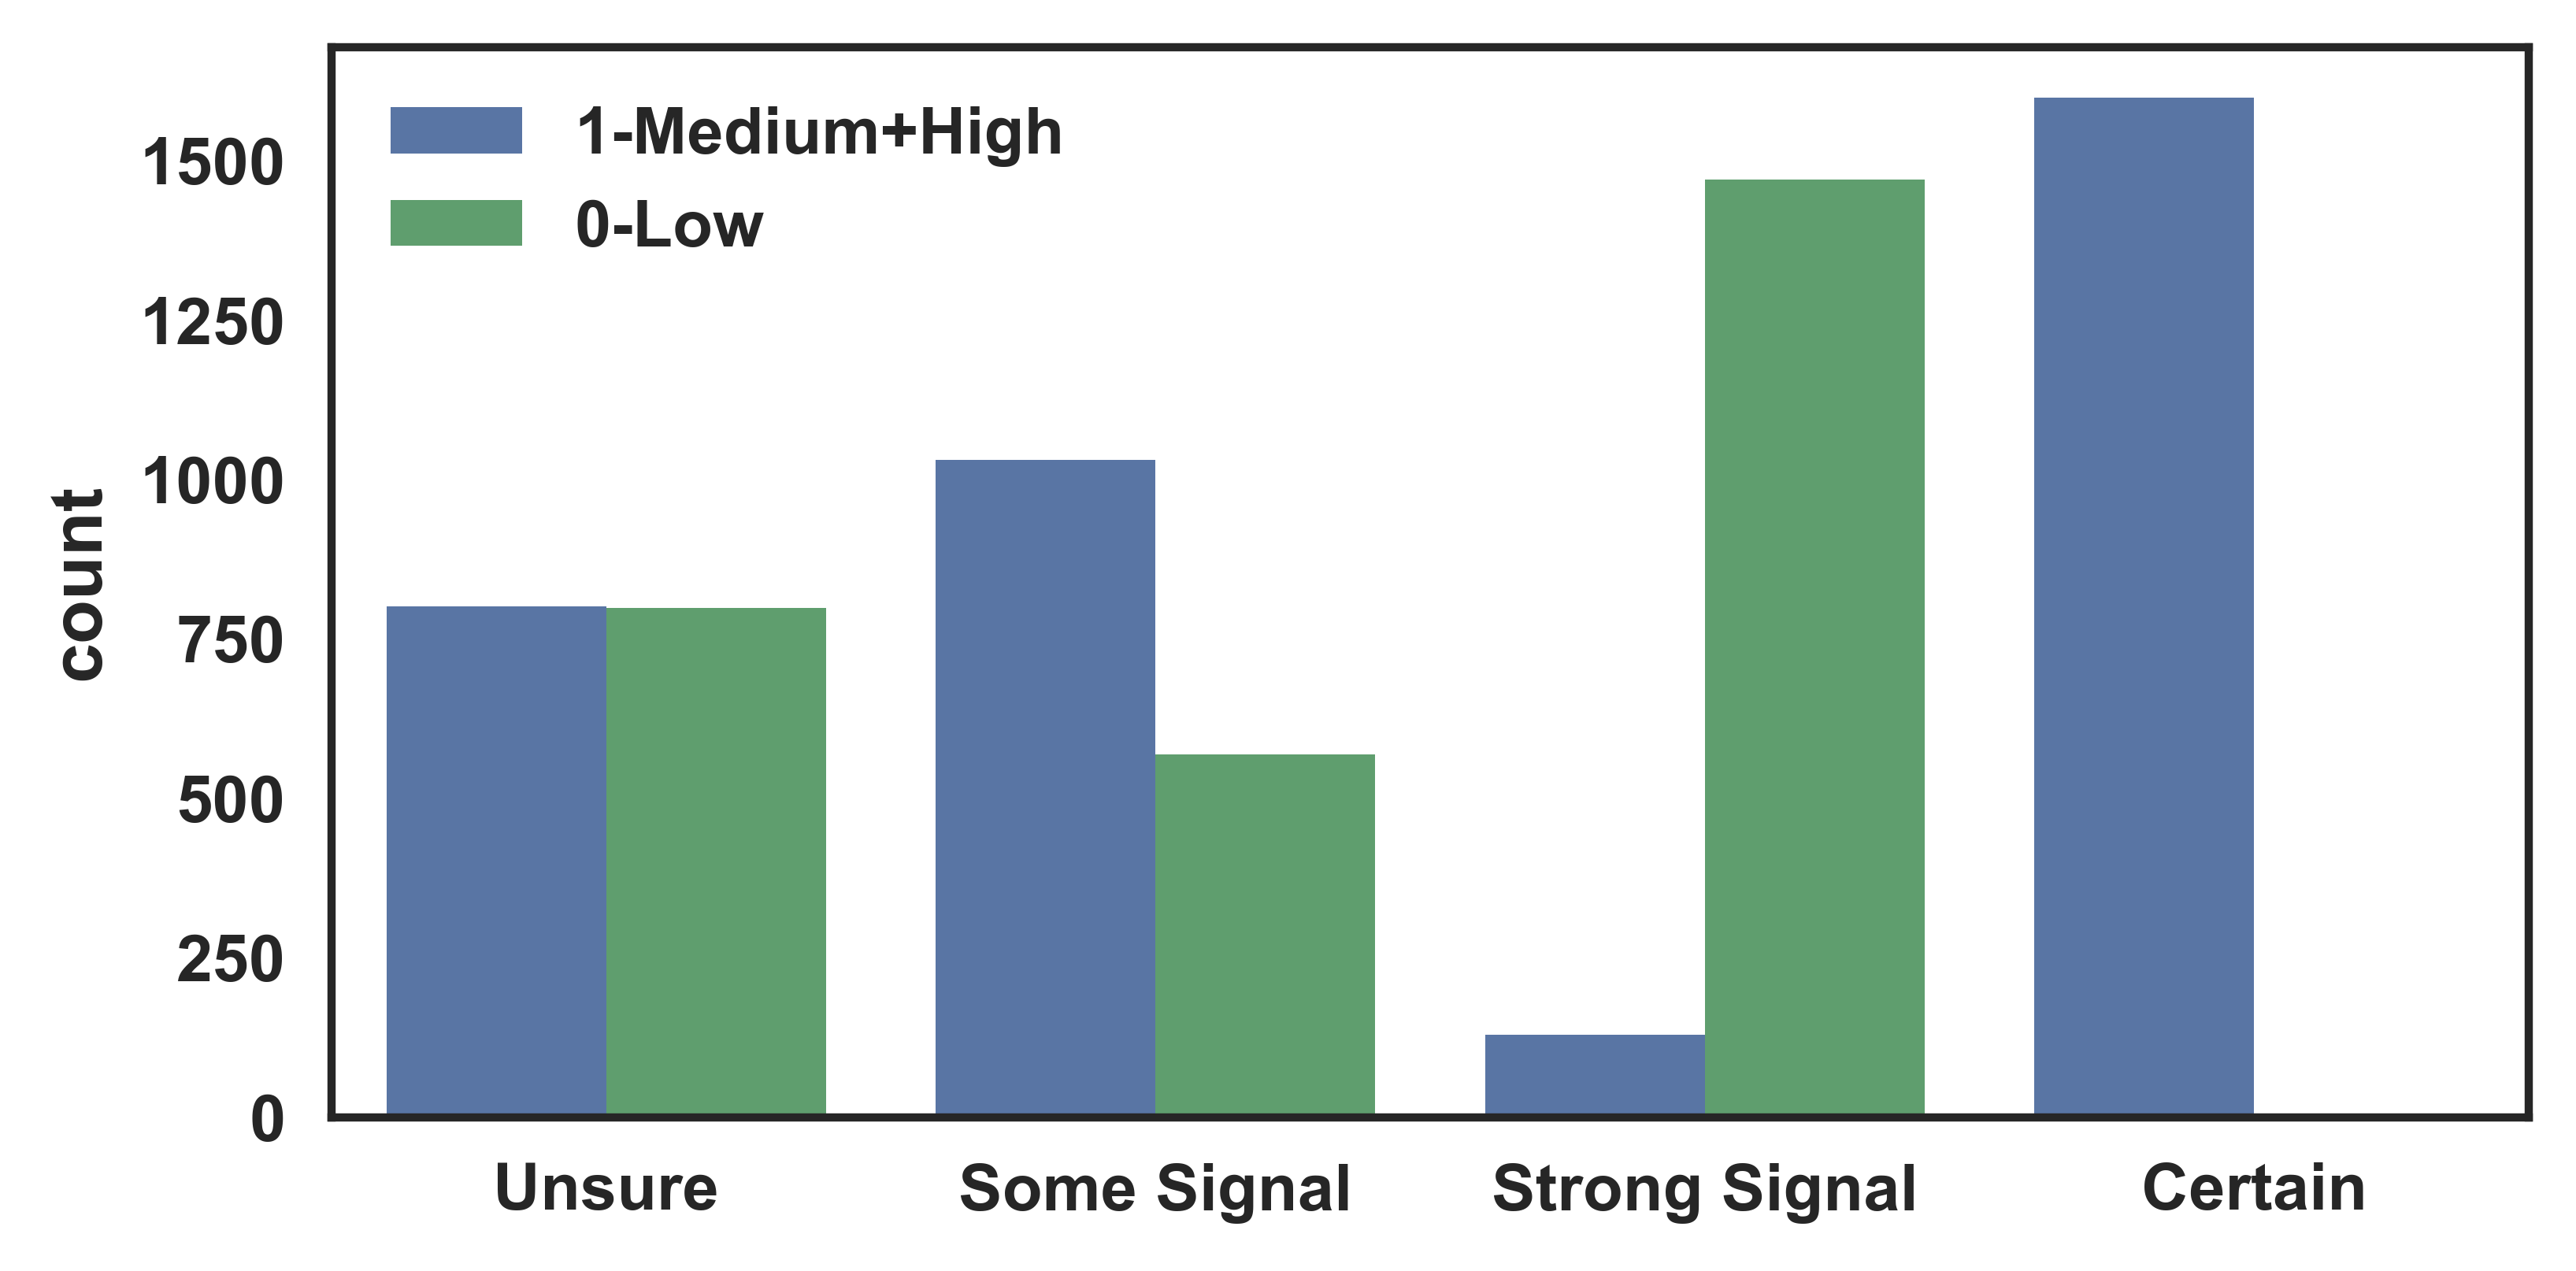
\includegraphics[width=0.95\columnwidth]{figures/prediction_ci.png}
	\caption{
		Uncertainty about out-of-sample predictions are demonstrated for 4 cases across the spectrum here. Since the model generates binary outcomes through MCMC simulation, if the split is 50-50, then the model is really not making any strong assertion - see the \textit{Unsure} case on the left. From left to right, the splits of the simulations get more pronounced, meaning in those predictive samples, the model is more and more certain of its prediction.
	}~\label{fig:pred_ci}	
	
	\centering
	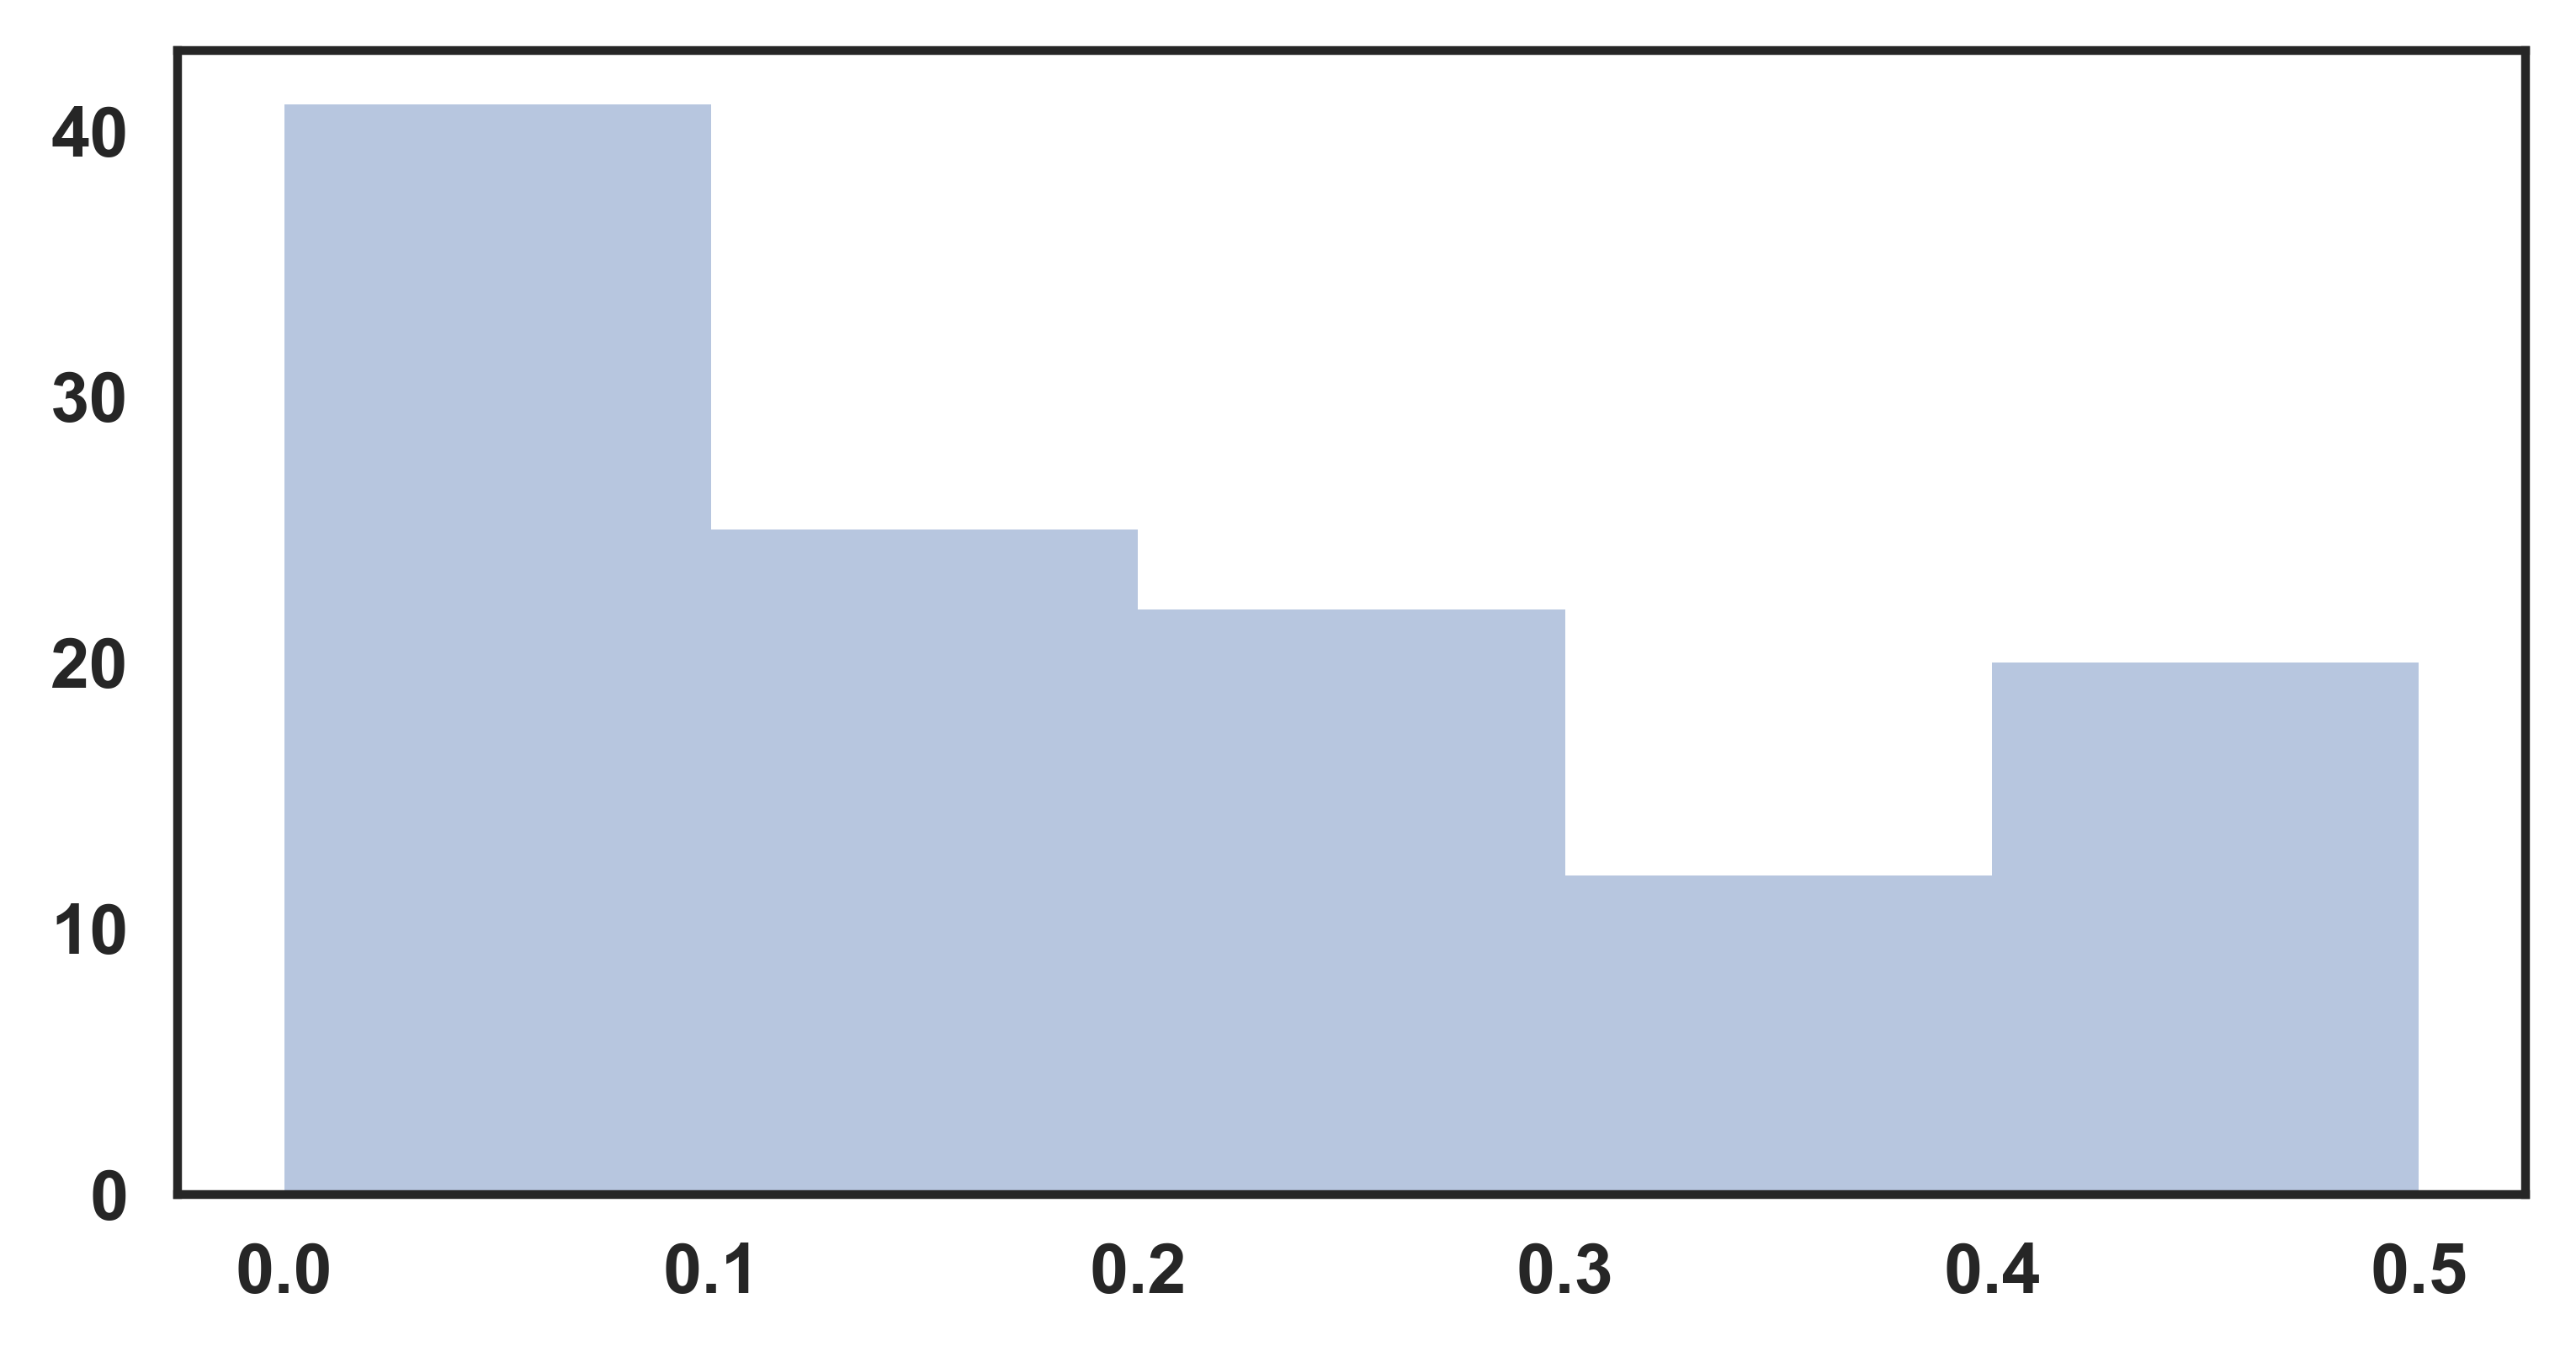
\includegraphics[width=0.95\columnwidth]{figures/prediction_se.png}
	\caption{
		This graph shows the empirical uncertainty of all 120 out-of-sample predictions, measured by standard errors. Notice that about 17pct of these samples have really high uncertainties (>0.4), which means the model almost refuses to classify these samples, and the assignment of these predictions in to classes are almost purely numerical noises.
	}~\label{fig:pred_se}	
	
\end{figure}


\subsection{Prediction confidence}
These hierarchical models are fitted using MCMC methods, so a distinctive advantage over black-box models is that each out-of-sample prediction comes with a whole distribution, which allows researchers to assess how confident the model is about a particular point estimate. Figures \ref{fig:pred_ci} and \ref{fig:pred_se} look deeper into different cases where the confidence varies.

The ability of this model to allow statistical inference on predictive cases are very useful, because it could aid users to \textbf{not} make a decision. For example, if the model is used to detect cheating or predict adverse drug reaction, refraining from making quick actions on uncertain predictions are almost always better than acting quickly on numerical noises (see Figure \ref{fig:pred_se}). 

 

\section{Conclusion}
This paper demonstrates that it is possible to build advanced
parametric models - \textbf{hierarchical models} in particular - that can outperform popular machine learning methods in prediction accuracy. Furthermore, hierarchical models also provides meaningful confidence intervals for statistical inference and decision making, which makes them well applicable to education research.

For future works, and extensions of the models built here with better assumptions and more informative priors could achieve even higher accuracy. Better methodology of model comparison and selection could also be further investigated. Alternatively, deeper inference into the fitted parameters could shed lights on the variability and differences of the groups in the hierarchy, which contributes further domain-specific insights to the educational research community.


\balance{}


% REFERENCES FORMAT
% References must be the same font size as other body text.
\bibliographystyle{SIGCHI-Reference-Format}
\bibliography{main}

\end{document}

%%% Local Variables:
%%% mode: latex
%%% TeX-master: t
%%% End:
